%% Please fill in your name and collaboration statement here.
\newcommand{\studentName}{**FILL IN YOUR NAME HERE**}
\newcommand{\collaborationStatement}{**FILL IN YOUR COLLABORATION STATEMENT HERE \\ (See the syllabus for information)**}


%%%%%%%%%%%%%%%%%%%%%%%%%%%%%%%%%%%%%%%%%%%%%%%
\documentclass[solution, letterpaper]{cs20inclass}
\usepackage{enumerate}
\usepackage{tikz}
\usepackage{pgf}
\usepackage{tikz}
\usepackage{hyperref}
\begin{document}
\header{4}{Monday, February 1, 2016}

\noindent Author: Tom Silver% \\


\paragraph*{Executive Summary}

\begin{enumerate}

\item Ordinary Induction
\begin{itemize}
\item A {\em predicate} is the statement you are trying to prove.
\item Let $P(x)$ be a predicate and $m, n$ nonnegative integers.  If $P(m)$ is true and $P(n) \Rightarrow P(n+1)$ for all $n \ge m$, then $P(n)$ is true for all $n \ge m$.

\item To write a proof by induction, first you need to identify the proposition to be proven.  Then prove the base case, prove the inductive step (how you can get from the proposition holding for $n$ to the proposition holding for $n+1$), and the conclusion.  Be sure you identify properly the thing being inducted upon.
\end{itemize}

\item Strong Induction
\begin{itemize}
\item In simple terms, strong induction is similar to ordinary induction, except you use $P(0)$, $\ldots$, $P(n)$ instead of just $P(n)$ in order to prove $P(n+1)$.
\item Formally, the difference between ordinary and strong induction is:\\
Let $P(x)$ be a predicate and $m,n$ nonnegative integers.
    \begin{itemize}
    \item Ordinary Induction: If $P(m)$ is true and $P(n) \Rightarrow P(n+1)$\\ for all $n \geq m$, then $P(n)$ is true for all $n      \geq m$.
    \item Strong Induction: If $P(m)$ is true and\\ $P(m), P(m+1), \dots, P(n)$ together $\Rightarrow P(n+1)$\\
    for all $n \geq m$, then $P(n)$ is true for all $n \geq m$.
    \end{itemize}
\item Strong induction proofs begin with the identification of the proposition to be proven. The next step is to identify and verify the base case. Note that with strong induction there are often multiple base cases. Next comes the inductive step, where you show that the proposition's truth for $0\ldots n$ entails its truth for $n+1$. Be sure to properly identify the proposition being inducted on.  
\item Note that sometimes you will need to break your inductive step into multiple cases.
\end{itemize}
\end{enumerate}

\problem

Using induction, prove that for all positive integers $n$:
$$
\sum_{k=1}^{n}\frac{1}{k(k+1)}=\frac{n}{n+1}
$$

\begin{solution}

TODO

\end{solution}

\problem

A tromino is an arrangement of three squares like the one shown below. It can be flipped and rotated in any direction. 

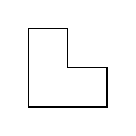
\begin{tikzpicture}[scale=0.5]

\draw (0,0) -- (2,0) -- (2,1) -- (1,1) -- (1,2) -- (0,2) -- (0,0);

\end{tikzpicture}

\subproblem

 Prove by induction that every $2^n \times 2^n$ grid with one corner removed can be covered with trominos. Example:

\begin{center}

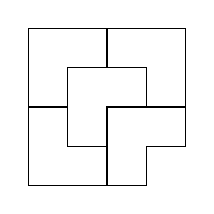
\begin{tikzpicture}[scale=0.5]

\draw (0,0) -- (3,0) -- (3,1) -- (4,1) -- (4,4) -- (0,4) -- (0,0);

\draw (2,0) -- (2,1) -- (1,1) -- (1,3) -- (3,3) -- (3,2) -- (2,2) -- (2,1);
\draw (0,2) -- (1,2);
\draw (2,4) -- (2,3);
\draw (3,2) -- (4,2);

\end{tikzpicture}
\end{center}

\subproblem

Explain how you can use the result from the previous part to prove that: 
\begin{center}
$2^{2n}-1$ is divisible by $3$, for all $n>0$
\end{center}

\begin{solution}

\subsolution TODO

\subsolution TODO 

\end{solution}

\problem 

(BONUS). You are putting together a jigsaw puzzle with $n \geq 1$ pieces. At each step you join together two matching pieces and produce a new (composite) piece. Prove by induction that no matter in which order you join the pieces, it takes $n-1$ steps to complete the puzzle. 

\begin{solution}

TODO

\end{solution}

\problem (BONUS) The Tower of Hanoi is a game with three poles and different sized circular disks, that looks like this:
\begin{center}
\includegraphics[width=10cm]{hanoi.jpg}
\end{center}
The objective of the game is to move the disks onto a different pole. There are two rules: you may only move one disk at once, and no disk may be placed on a pole with a smaller disk beneath it. Prove that a Tower of Hanoi with $n$ disks takes $2^n-1$ to solve.
\begin{solution}

TODO
 
\end{solution}

\end{document}
